\begin{fact}\label{iso-tri-one-side-fixed}
	Considérons tous les triangles de périmètre fixé $p$, et ayant tous au moins un côté de même mesure $c$ (on suppose que nous avons au moins un tel triangle).
	Parmi tous ces triangles, celui qui a une aire maximale est le triangle isocèle ayant une base de mesure $c$.
\end{fact}


\begin{proof}
	Soit $ABC$ un triangle de périmètre $p$, et vérifiant $AB = c$. Les points $M$ sur la parallèle à $(AB)$ passant par $C$ sont tels que $\area{ABM} = \area{ABC}$. On note $O$ le point sur cette parallèle tel que $ABO$ soit isocèle en $O$.

	\begin{center}
		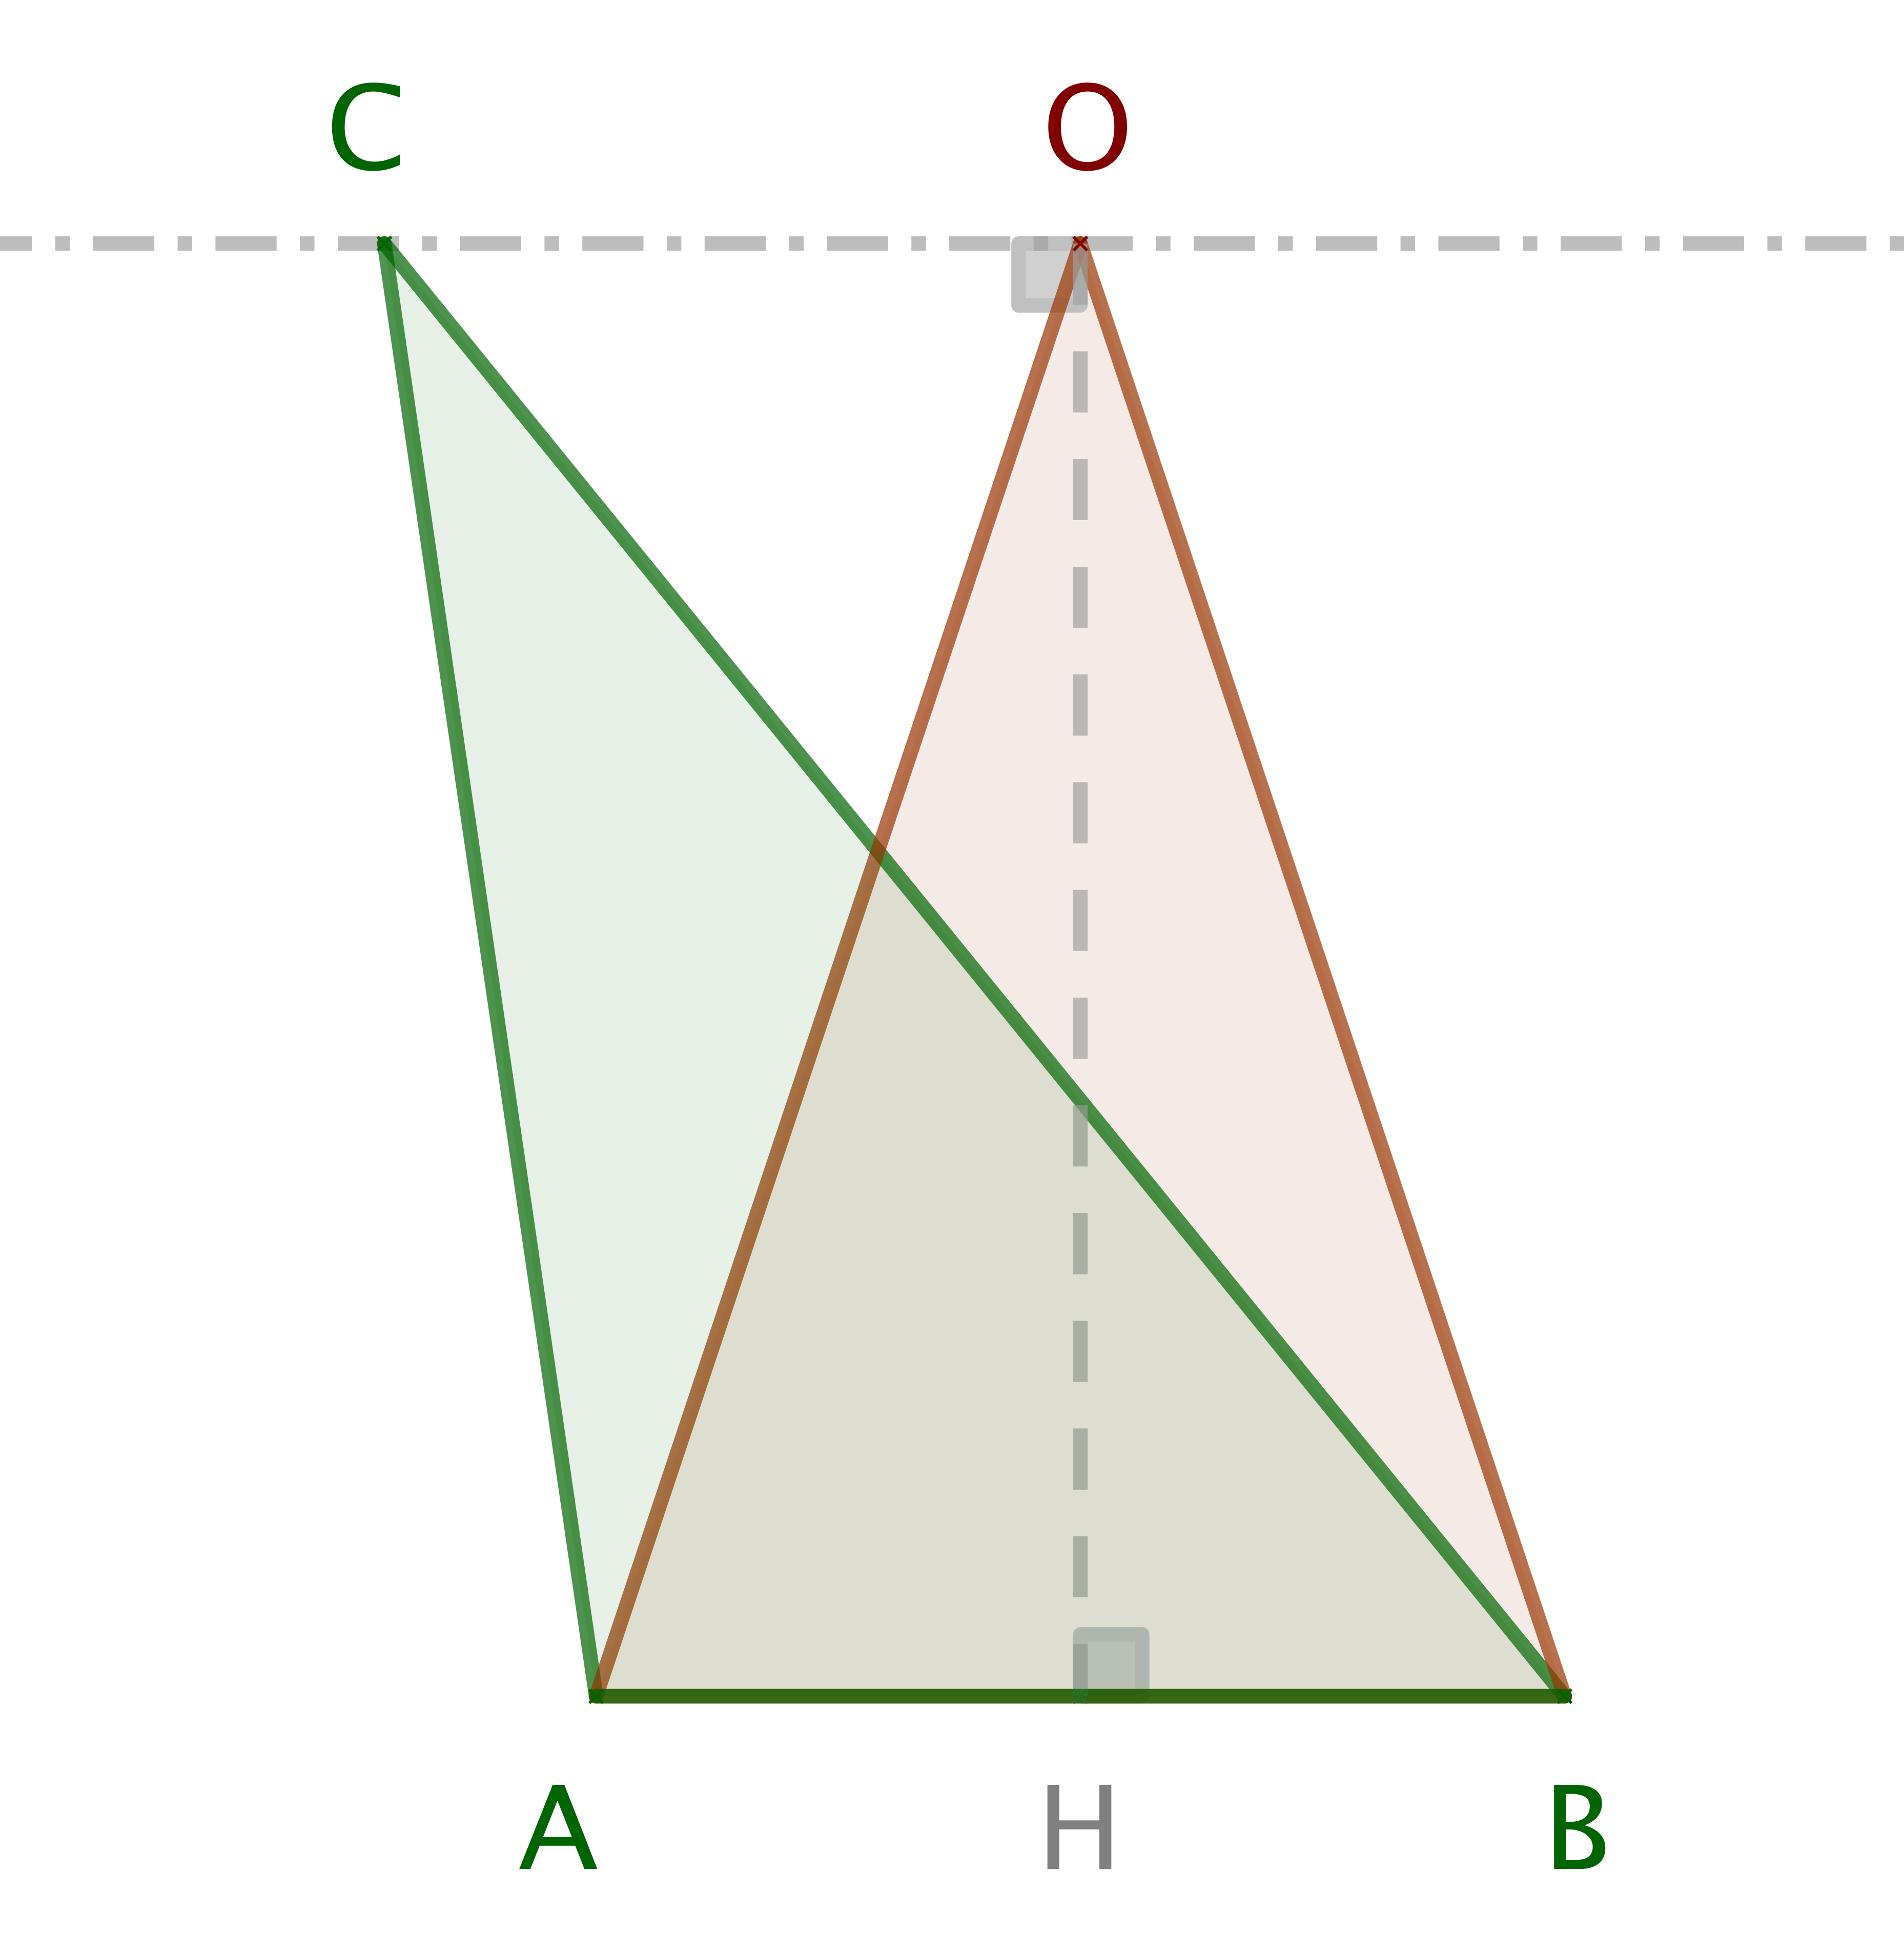
\includegraphics[scale=.4]{content/triangle-one-side-fixed/triangle.png}
	\end{center}

	
	Via une petite symétrie axiale, voir ci-dessous, il est aisé de noter que $\perim{ABC} \geq \perim{ABO}$.
	
	\begin{center}
		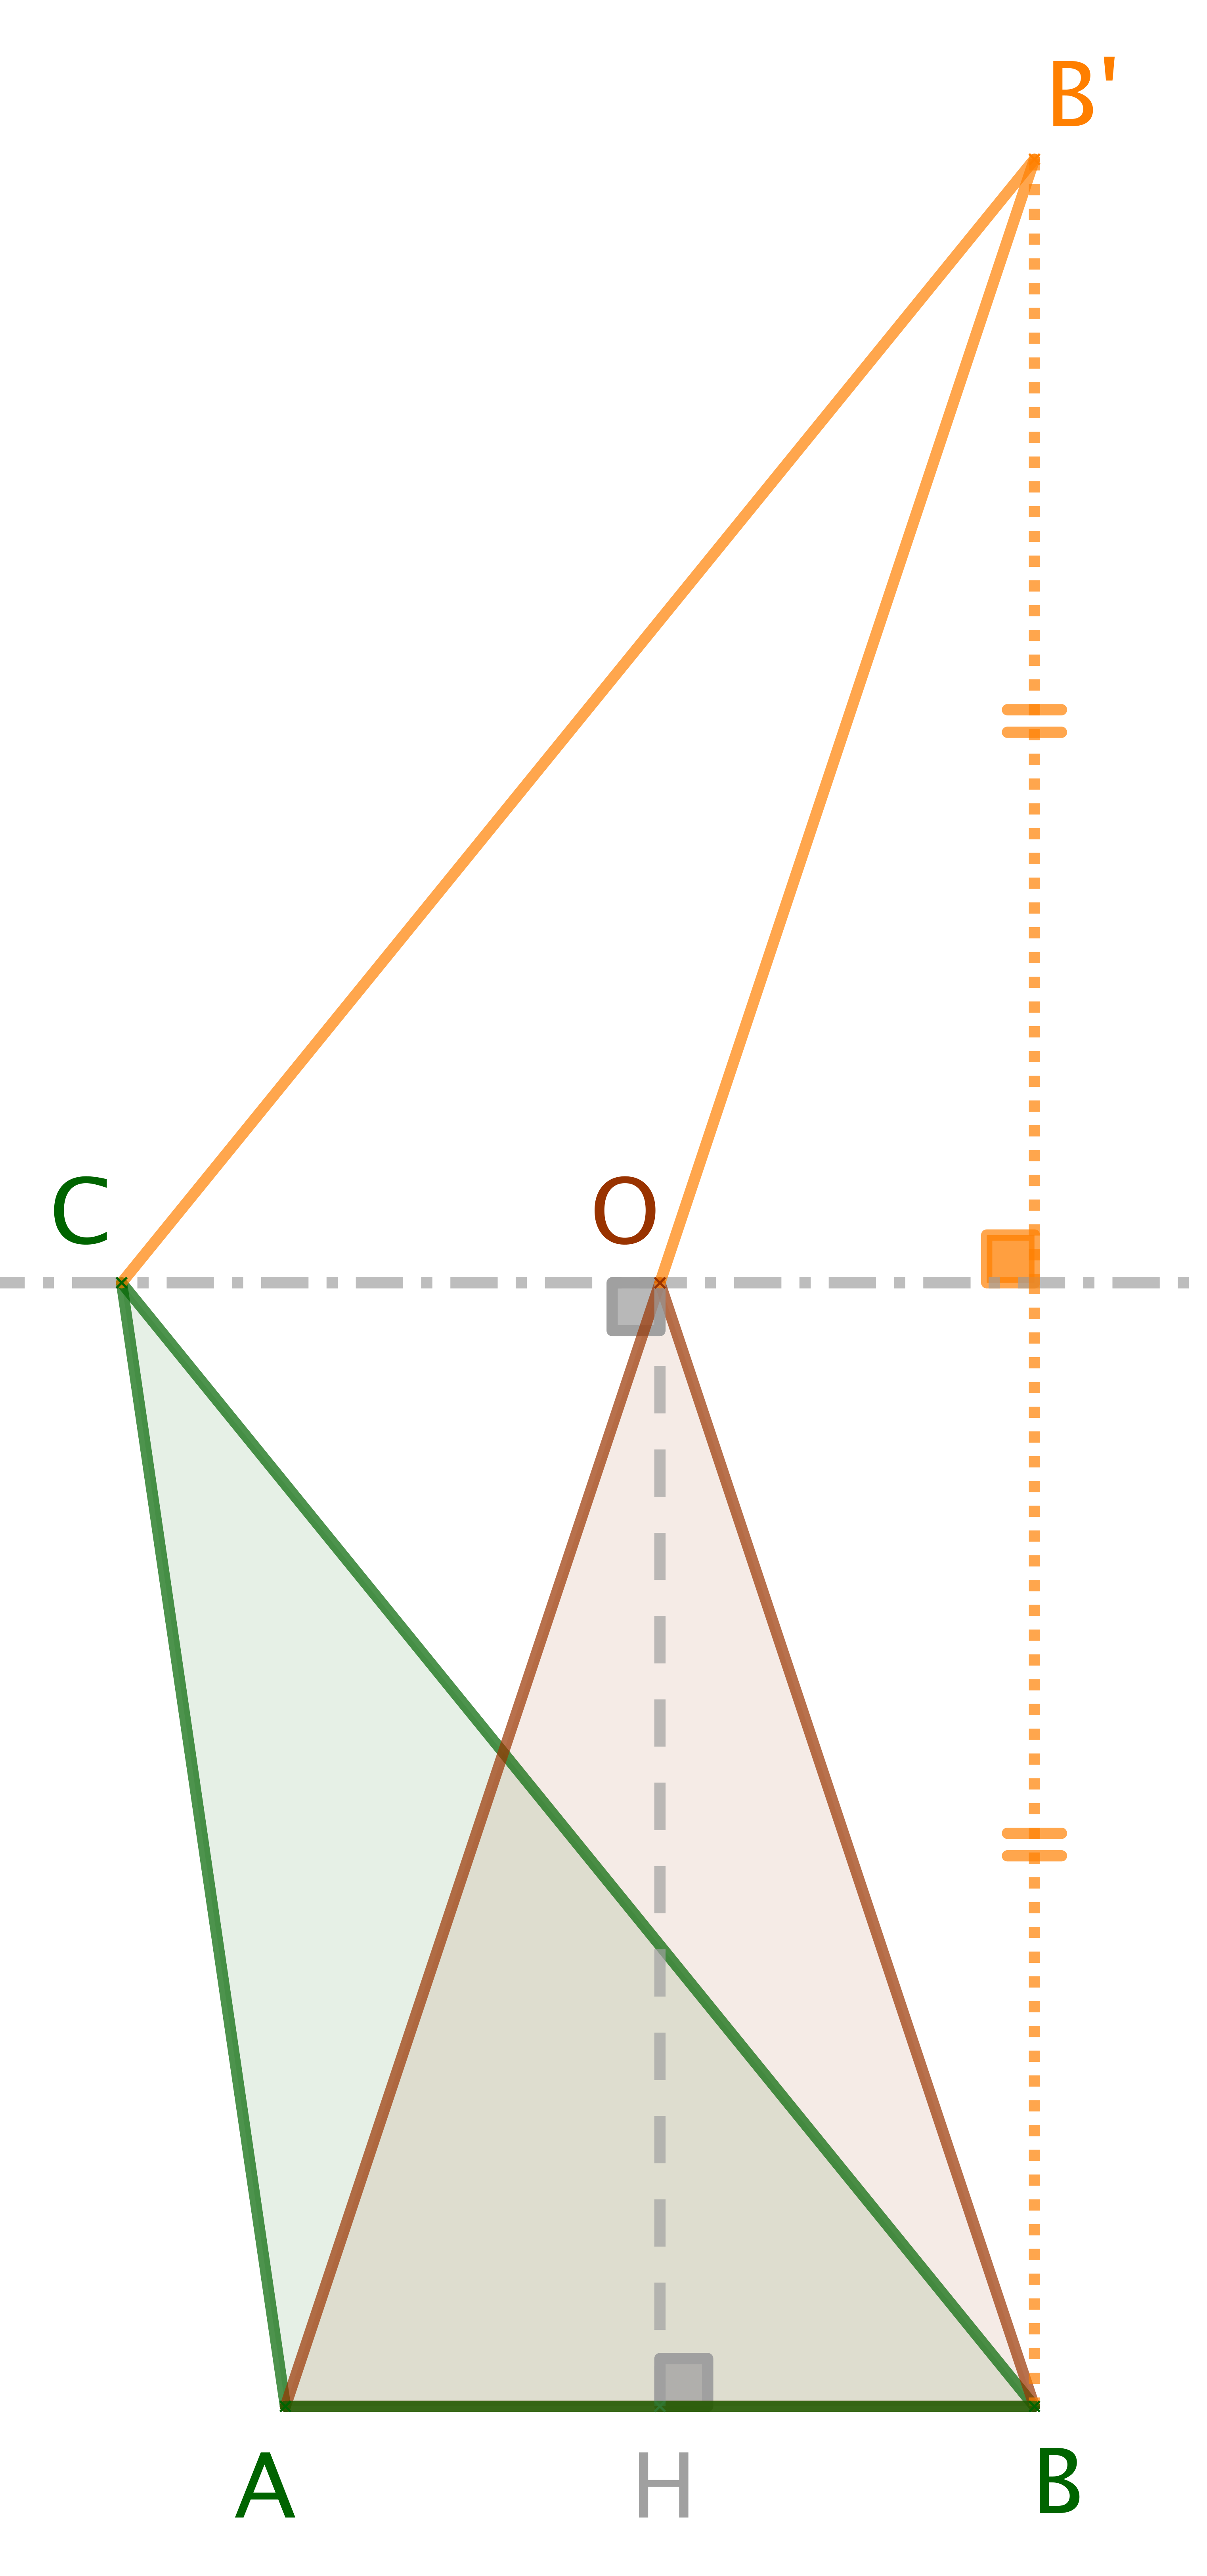
\includegraphics[scale=.4]{content/triangle-one-side-fixed/triangle-proof.png}
	\end{center}
	
	Via une dilatation \og \emph{verticale} \fg\ de rapport $r = \frac{\perim{ABC}}{\perim{ABO}} \geq 1$, on obtient finalement un triangle isocèle $ABO^{\,\prime}$ de périmètre $p$, et qui vérifie $\area{ABO^{\,\prime}} \geq \area{ABC}$.
	\footnote{
		Il est immédiat d'adapter les arguments de la méthode des extrema liés pour le triangle général au cas qui nous a occupé dans cette preuve.
	}
	Contrat rempli!
\end{proof}